\documentclass[16 pt]{amsart}
\usepackage{amscd,amsmath,amsthm,amssymb}
\usepackage{enumerate,varioref}
\usepackage{epsfig}
\usepackage{graphicx}
\usepackage{mathtools}
\usepackage{tikz}
\usepackage{amsfonts}
\usepackage{svg}
\usetikzlibrary{graphs,arrows,topaths}
\newtheorem{thm}{Theorem}
\newtheorem{cor}[thm]{Corollary}
\newtheorem{lem}[thm]{Lemma}
\newtheorem{prop}[thm]{Proposition}
\theoremstyle{definition}
\newtheorem{defn}[thm]{Definition}
\theoremstyle{remark}
\newtheorem{ex}[thm]{Example}
\newtheorem{rem}[thm]{Remark}
\numberwithin{equation}{subsection}
\newcommand{\R}{\mathbb{R}}
\newcommand{\Z}{\mathbb{Z}}
\newcommand{\C}{\mathbb{C}}
\newcommand{\Q}{\mathbb{Q}}
\begin{document}

\title{Homework 6 Maths 140 Winter 2015}
\maketitle 

10.5.3: What is the total degree of a tree with n vertices? Why?

\vspace{1in}

Solution: We simply apply two theorems here.  First, we have the handshake theorem which states that the degree of a graph is exactly twice the number of edges.  Second we have a theorem about trees which says that the total number of edges is eactly one less than the number of vertices.

\[
(1) deg(G) = 2|E(G)|, \text{ and } (2) |E(T)| = |V(T)|-1
\]

So in total we have for a tree $T$ with $n$ vertices
\[
deg(T) = 2|E(T)| = 2(|V(T)|-1) = 2(n-1) = 2n-2.
\]

\newpage

10.5.16: Draw a graph which is a tree with 12 vertices and 15 edges or explain why such a graph does not exist.

\vspace{1in}

Solution:  Judging from the problem above a tree with 12 vertices must have 11 edges.  So this graph cannot be drawn.

\newpage

10.5. 28: Is a circuit free graph with $n$ vertices and at least $n-1$ edges connected? Why?

\vspace{1in}

Solution: This is a essentially the definition of a tree.  If a graph has more than $n-1$ edges then it has a circuit.  If a graph has fewer than $n-1$ edges then is it not connected.  Therefore, a circuit free graph with at least $n-1$ edges will have exactly $n-1$ edges.  If this graph is not connected then we would look at all the connected components.  Each one must be a tree since the graph is circuit free.  Thus for each connected component we have $k-1$ edges where $k$ is the number of vertices in the connected component.  If we have more than one component then the total number of edges will be no greater than $n-2$, which contradicts our assumption.  Therefore any circuit free graph with $n$ vertices and $n-1$ edges is a tree.

\newpage

10.6.15: Draw a full binary tree with four internal vertices.

\vspace{1in}

Solution:

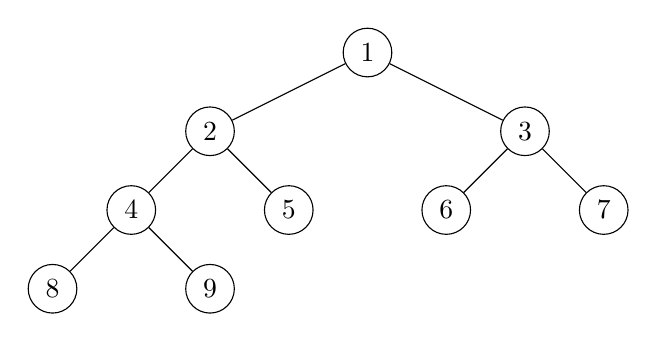
\begin{tikzpicture}
\node[circle,draw] (1) at (4,3){1};
\node[circle,draw] (2) at (2,2){2};
\node[circle,draw] (3) at (6,2){3};
\node[circle,draw] (4) at (1,1){4};
\node[circle,draw] (5) at (3,1){5};
\node[circle,draw] (6) at (5,1){6};
\node[circle,draw] (7) at (7,1){7};
\node[circle,draw] (8) at (0,0){8};
\node[circle,draw] (9) at (2,0){9};
\foreach \from/\to in {1/2,1/3,2/4,2/5,3/6,3/7,4/8,4/9}
  \draw (\from) -- (\to);
\end{tikzpicture}

\newpage

10.6.19: Draw a full binary, heIght 3, seven terminal vertices

\vspace{1in}

Solution:

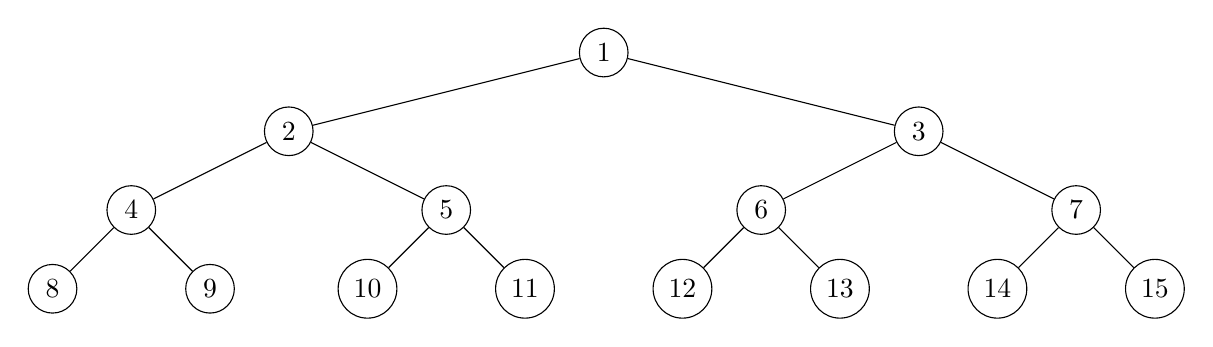
\begin{tikzpicture}
\node[circle,draw] (1) at (7,3){1};
\node[circle,draw] (2) at (3,2){2};
\node[circle,draw] (3) at (11,2){3};
\node[circle,draw] (4) at (1,1){4};
\node[circle,draw] (5) at (5,1){5};
\node[circle,draw] (6) at (9,1){6};
\node[circle,draw] (7) at (13,1){7};
\node[circle,draw] (8) at (0,0){8};
\node[circle,draw] (9) at (2,0){9};
\node[circle,draw] (10) at (4,0){10};
\node[circle,draw] (11) at (6,0){11};
\node[circle,draw] (12) at (8,0){12};
\node[circle,draw] (13) at (10,0){13};
\node[circle,draw] (14) at (12,0){14};
\node[circle,draw] (15) at (14,0){15};
\foreach \from/\to in {1/2,1/3,2/4,2/5,3/6,3/7,4/8,4/9,5/10,5/11,6/12,6/13,7/14,7/15}
  \draw (\from) -- (\to);
\end{tikzpicture}


\end{document}